% Options for packages loaded elsewhere
\PassOptionsToPackage{unicode}{hyperref}
\PassOptionsToPackage{hyphens}{url}
\PassOptionsToPackage{dvipsnames,svgnames,x11names}{xcolor}
%
\documentclass[
  a4paper,
  DIV=11,
  numbers=noendperiod]{scrartcl}

\usepackage{amsmath,amssymb}
\usepackage{iftex}
\ifPDFTeX
  \usepackage[T1]{fontenc}
  \usepackage[utf8]{inputenc}
  \usepackage{textcomp} % provide euro and other symbols
\else % if luatex or xetex
  \usepackage{unicode-math}
  \defaultfontfeatures{Scale=MatchLowercase}
  \defaultfontfeatures[\rmfamily]{Ligatures=TeX,Scale=1}
\fi
\usepackage{lmodern}
\ifPDFTeX\else  
    % xetex/luatex font selection
\fi
% Use upquote if available, for straight quotes in verbatim environments
\IfFileExists{upquote.sty}{\usepackage{upquote}}{}
\IfFileExists{microtype.sty}{% use microtype if available
  \usepackage[]{microtype}
  \UseMicrotypeSet[protrusion]{basicmath} % disable protrusion for tt fonts
}{}
\makeatletter
\@ifundefined{KOMAClassName}{% if non-KOMA class
  \IfFileExists{parskip.sty}{%
    \usepackage{parskip}
  }{% else
    \setlength{\parindent}{0pt}
    \setlength{\parskip}{6pt plus 2pt minus 1pt}}
}{% if KOMA class
  \KOMAoptions{parskip=half}}
\makeatother
\usepackage{xcolor}
\setlength{\emergencystretch}{3em} % prevent overfull lines
\setcounter{secnumdepth}{-\maxdimen} % remove section numbering
% Make \paragraph and \subparagraph free-standing
\makeatletter
\ifx\paragraph\undefined\else
  \let\oldparagraph\paragraph
  \renewcommand{\paragraph}{
    \@ifstar
      \xxxParagraphStar
      \xxxParagraphNoStar
  }
  \newcommand{\xxxParagraphStar}[1]{\oldparagraph*{#1}\mbox{}}
  \newcommand{\xxxParagraphNoStar}[1]{\oldparagraph{#1}\mbox{}}
\fi
\ifx\subparagraph\undefined\else
  \let\oldsubparagraph\subparagraph
  \renewcommand{\subparagraph}{
    \@ifstar
      \xxxSubParagraphStar
      \xxxSubParagraphNoStar
  }
  \newcommand{\xxxSubParagraphStar}[1]{\oldsubparagraph*{#1}\mbox{}}
  \newcommand{\xxxSubParagraphNoStar}[1]{\oldsubparagraph{#1}\mbox{}}
\fi
\makeatother


\providecommand{\tightlist}{%
  \setlength{\itemsep}{0pt}\setlength{\parskip}{0pt}}\usepackage{longtable,booktabs,array}
\usepackage{calc} % for calculating minipage widths
% Correct order of tables after \paragraph or \subparagraph
\usepackage{etoolbox}
\makeatletter
\patchcmd\longtable{\par}{\if@noskipsec\mbox{}\fi\par}{}{}
\makeatother
% Allow footnotes in longtable head/foot
\IfFileExists{footnotehyper.sty}{\usepackage{footnotehyper}}{\usepackage{footnote}}
\makesavenoteenv{longtable}
\usepackage{graphicx}
\makeatletter
\def\maxwidth{\ifdim\Gin@nat@width>\linewidth\linewidth\else\Gin@nat@width\fi}
\def\maxheight{\ifdim\Gin@nat@height>\textheight\textheight\else\Gin@nat@height\fi}
\makeatother
% Scale images if necessary, so that they will not overflow the page
% margins by default, and it is still possible to overwrite the defaults
% using explicit options in \includegraphics[width, height, ...]{}
\setkeys{Gin}{width=\maxwidth,height=\maxheight,keepaspectratio}
% Set default figure placement to htbp
\makeatletter
\def\fps@figure{htbp}
\makeatother
% definitions for citeproc citations
\NewDocumentCommand\citeproctext{}{}
\NewDocumentCommand\citeproc{mm}{%
  \begingroup\def\citeproctext{#2}\cite{#1}\endgroup}
\makeatletter
 % allow citations to break across lines
 \let\@cite@ofmt\@firstofone
 % avoid brackets around text for \cite:
 \def\@biblabel#1{}
 \def\@cite#1#2{{#1\if@tempswa , #2\fi}}
\makeatother
\newlength{\cslhangindent}
\setlength{\cslhangindent}{1.5em}
\newlength{\csllabelwidth}
\setlength{\csllabelwidth}{3em}
\newenvironment{CSLReferences}[2] % #1 hanging-indent, #2 entry-spacing
 {\begin{list}{}{%
  \setlength{\itemindent}{0pt}
  \setlength{\leftmargin}{0pt}
  \setlength{\parsep}{0pt}
  % turn on hanging indent if param 1 is 1
  \ifodd #1
   \setlength{\leftmargin}{\cslhangindent}
   \setlength{\itemindent}{-1\cslhangindent}
  \fi
  % set entry spacing
  \setlength{\itemsep}{#2\baselineskip}}}
 {\end{list}}
\usepackage{calc}
\newcommand{\CSLBlock}[1]{\hfill\break\parbox[t]{\linewidth}{\strut\ignorespaces#1\strut}}
\newcommand{\CSLLeftMargin}[1]{\parbox[t]{\csllabelwidth}{\strut#1\strut}}
\newcommand{\CSLRightInline}[1]{\parbox[t]{\linewidth - \csllabelwidth}{\strut#1\strut}}
\newcommand{\CSLIndent}[1]{\hspace{\cslhangindent}#1}

\KOMAoption{captions}{tableheading}
\makeatletter
\@ifpackageloaded{caption}{}{\usepackage{caption}}
\AtBeginDocument{%
\ifdefined\contentsname
  \renewcommand*\contentsname{Table of contents}
\else
  \newcommand\contentsname{Table of contents}
\fi
\ifdefined\listfigurename
  \renewcommand*\listfigurename{List of Figures}
\else
  \newcommand\listfigurename{List of Figures}
\fi
\ifdefined\listtablename
  \renewcommand*\listtablename{List of Tables}
\else
  \newcommand\listtablename{List of Tables}
\fi
\ifdefined\figurename
  \renewcommand*\figurename{Figure}
\else
  \newcommand\figurename{Figure}
\fi
\ifdefined\tablename
  \renewcommand*\tablename{Table}
\else
  \newcommand\tablename{Table}
\fi
}
\@ifpackageloaded{float}{}{\usepackage{float}}
\floatstyle{ruled}
\@ifundefined{c@chapter}{\newfloat{codelisting}{h}{lop}}{\newfloat{codelisting}{h}{lop}[chapter]}
\floatname{codelisting}{Listing}
\newcommand*\listoflistings{\listof{codelisting}{List of Listings}}
\makeatother
\makeatletter
\makeatother
\makeatletter
\@ifpackageloaded{caption}{}{\usepackage{caption}}
\@ifpackageloaded{subcaption}{}{\usepackage{subcaption}}
\makeatother

\ifLuaTeX
\usepackage[bidi=basic]{babel}
\else
\usepackage[bidi=default]{babel}
\fi
\babelprovide[main,import]{american}
% get rid of language-specific shorthands (see #6817):
\let\LanguageShortHands\languageshorthands
\def\languageshorthands#1{}
\ifLuaTeX
  \usepackage{selnolig}  % disable illegal ligatures
\fi
\usepackage{bookmark}

\IfFileExists{xurl.sty}{\usepackage{xurl}}{} % add URL line breaks if available
\urlstyle{same} % disable monospaced font for URLs
\hypersetup{
  pdftitle={Analog Circuit Design},
  pdfauthor={Harald Pretl},
  pdflang={en-US},
  colorlinks=true,
  linkcolor={blue},
  filecolor={Maroon},
  citecolor={Blue},
  urlcolor={Blue},
  pdfcreator={LaTeX via pandoc}}


\title{Analog Circuit Design}
\author{Harald Pretl}
\date{2024-08-01}

\begin{document}
\maketitle

\renewcommand*\contentsname{Table of contents}
{
\hypersetup{linkcolor=}
\setcounter{tocdepth}{3}
\tableofcontents
}

\subsection{Introduction}\label{sec-intro}

This is the material for an intermediate-level MOSFET circuit design
course, held at JKU under course number 336.009 (``KV Analoge
Schaltungstechnik'').

The course makes heavy use of circuit simulation, using \textbf{Xschem}
for schematic entry and \textbf{ngspice} for simulation. The 130nm CMOS
technology \textbf{SG13G2} from IHP Microelectronics is used.

Tools and PDK are integrated in the \textbf{IIC-OSIC-TOOLS} Docker
image, which will be used during the coursework.

All course material is made publicly available and shared under the
Apache-2.0 license.

\subsubsection{IHP's SG13G2 130nm CMOS
Technology}\label{ihps-sg13g2-130nm-cmos-technology}

SG13G2 is the name of a 130nm CMOS technology (strictly speaking BiCMOS)
from IHP Microelectronics. It features low-voltage (thin-oxide) core
MOSFET, high-voltage (thick-oxide) I/O MOSFET, various types of linear
resistors, and 7 layers of Aluminium metallization (5 thin, 2 thick
metal layers). This PDK is open-source, and the complete process
specification can be found at
\href{https://github.com/IHP-GmbH/IHP-Open-PDK/blob/main/ihp-sg13g2/libs.doc/doc/SG13G2_os_process_spec.pdf}{SG13G2
process specification}. While we will not do layouts in this course, the
layout rules can be found at
\href{https://github.com/IHP-GmbH/IHP-Open-PDK/blob/main/ihp-sg13g2/libs.doc/doc/SG13G2_os_layout_rules.pdf}{SG13G2
layout rules}.

For our circuit design, the most important parameters of the available
devices are summarized in the following:

\begin{itemize}
\tightlist
\item
  \textbf{Low-voltage NMOS}: Device \texttt{sg13\_lv\_nmos}; operating
  voltage nominal \(V_\mathrm{DD}=1.5\,\text{V}\),
  \(L_\mathrm{min}=0.13\,\mu\text{m}\),
  \(V_\mathrm{th} \approx 0.5\,\text{V}\); a triple-well option for the
  NMOS is available.
\item
  \textbf{Low-voltage PMOS}: Device \texttt{sg13\_lv\_pmos}; operating
  voltage nominal \(V_\mathrm{DD}=1.5\,\text{V}\),
  \(L_\mathrm{min}=0.13\,\mu\text{m}\),
  \(V_\mathrm{th} \approx -0.47\,\text{V}\).
\item
  \textbf{High-voltage NMOS}: Device \texttt{sg13\_hv\_nmos}; operating
  voltage nominal \(V_\mathrm{DD}=3.3\,\text{V}\),
  \(L_\mathrm{min}=0.45\,\mu\text{m}\),
  \(V_\mathrm{th} \approx 0.7\,\text{V}\); a triple-well option for the
  NMOS is available.
\item
  \textbf{High-voltage PMOS}: Device \texttt{sg13\_hv\_pmos}; operating
  voltage nominal \(V_\mathrm{DD}=3.3\,\text{V}\),
  \(L_\mathrm{min}=0.45\,\mu\text{m}\),
  \(V_\mathrm{th} \approx -0.65\,\text{V}\).
\item
  \textbf{Silicided poly resistor}: Device \texttt{rsil};
  \(R_\square=7\,\Omega \pm 10\%\), \(\mathrm{TC}_1=3100\,\text{ppm/K}\)
\item
  \textbf{Poly resistor}: Device \texttt{rppd};
  \(R_\square=260\,\Omega \pm 10\%\),
  \(\mathrm{TC}_1=170\,\text{ppm/K}\)
\item
  \textbf{Poly resistor high}: Device \texttt{rhigh};
  \(R_\square=1360\,\Omega \pm 15\%\),
  \(\mathrm{TC}_1=-2300\,\text{ppm/K}\)
\item
  \textbf{MIM capacitor}: Device \texttt{cap\_cmim};
  \(C'=1.5\,\text{fF}/\mu\text{m}^2 \pm 10\%\),
  \(\mathrm{VC}_1=-26\text{ppm/V}\), \(\mathrm{TC}_1=3.6\text{ppm/K}\),
  breakdown voltage \(>15\,\mathrm{V}\)
\item
  \textbf{MOM capacitor}: Well-suited metal stack due to 5 thin metal
  layers, but no primitive capacitor available.
\end{itemize}

\subsubsection{Schematic Entry Using
Xschem}\label{schematic-entry-using-xschem}

Xschem is an open-source schematic entry tool with emphasis on
integrated circuits. For up-to-date information of the many features of
Xschem please look at the
\href{https://xschem.sourceforge.io/stefan/xschem_man/xschem_man.html}{online
documentation}. Usage of Xschem will be learned with the first few basic
examples, essentially a single MOSFET. The usage model of Xschem is that
the schematic is hierarchically drawn, and the simulation and evaluation
statements are contained in the schematics. Further, Xschem offers
embedded graphing, which we will mostly use.

\subsubsection{Circuit Simulation Using
ngspice}\label{circuit-simulation-using-ngspice}

ngspice is an open-source circuit simulator with SPICE dependency.
Besides the usual simulated types like \texttt{op} (operating point),
\texttt{dc} (dc sweeps), \texttt{tran} (time-domain), or \texttt{ac}
(for small-signal frquency sweeps), ngspice offers a script-like control
interface, where many different simulation controls and result
evaluations can be done. For detailed information please refer to the
latest
\href{https://ngspice.sourceforge.io/docs/ngspice-43-manual.pdf}{manual}.

\subsubsection{Integrated IC Design Environment
(IIC-OSIC-TOOLS)}\label{integrated-ic-design-environment-iic-osic-tools}

In order to make usage of the various required components (tools like
Xschem, PDK like SG13G2) easier, we will use the IIC-OSIC-TOOLS. This is
a pre-setup Docker image which allows to design on a virtual machine on
virtually any type of computing equipment. For further information like
installed tools, how to setup a VM, etc. please look at
\href{https://github.com/iic-jku/IIC-OSIC-TOOLS}{IIC-OSIC-TOOLS GitHub
page}.

Experienced users can install this image on their personal computer, for
JKU students the IIC will host a VM on our compute cluster and provide
personal login credentials.

\subsection{First Steps}\label{first-steps}

In this first chapter we will learn to use Xschem for schematic entry,
and how to operate the ngspice SPICE simulator for circuit simulations.
Further, we will make ourself familiar with the transistor and other
passive components available in the IHP Microelectronics SG13G2
technology. While this is strictly speaking a BiCMOS technology offering
MOSFETs as well as SiGe HBTs, we will use it as a pure CMOS technology.

\subsubsection{The Metal-Oxide-Semiconductor Field-Effect-Transistor
(MOSFET)}\label{sec-mosfet}

In this course, we will not dive into semiconductor physics and derive
the device operation bottom-up starting from a fundamental level
governed by quantum mechanics. Instead, we will treat the MOSFET
macroscopic by assuming we have a 4-terminal device, and the performance
of this device regarding its terminal voltages and currents we will
largely derive from the simulation model. For hand calculations and
theoretical discussions we will use the following simplified
large-signal model.

\begin{figure}[H]

\centering{

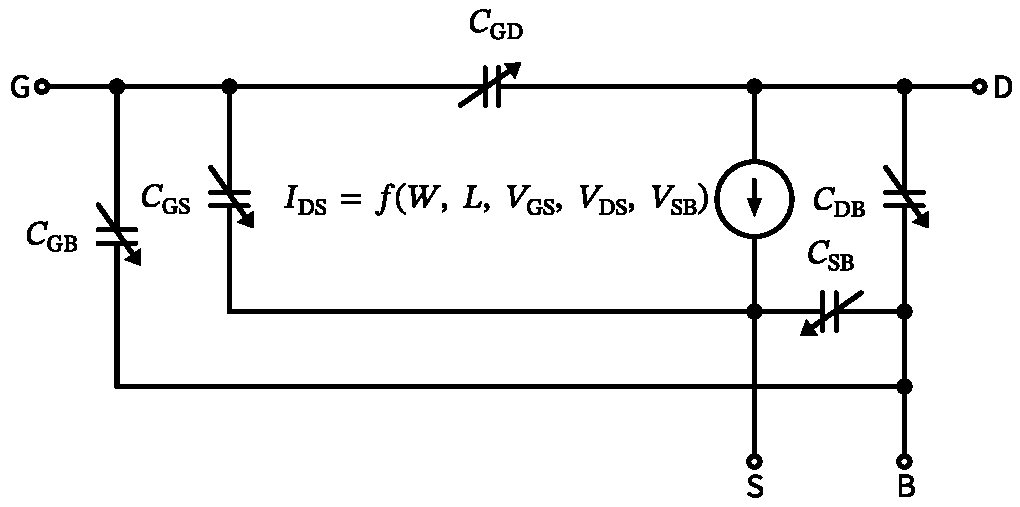
\includegraphics{index_files/mediabag/index_files/figure-pdf/fig-mosfet-large-signal-model-output-1.pdf}

}

\caption{\label{fig-mosfet-large-signal-model}The MOSFET large-signal
model.}

\end{figure}%

\textsubscript{Source:
\href{https://iic-jku.github.io/analog-circuit-design/index.qmd.html}{Article
Notebook}}

A first step in any new IC technology should be to investigate basic
MOSFET performance, by doing simple dc sweeps of \(V_\mathrm{GS}\) and
\(V_\mathrm{DS}\) and looking at \(I_\mathrm{DS}\) and other large- and
small-signal parameters.

As this is an intermediate-level course, some basic knowledge about
MOSFET operation, basic device equations, and small-signal equivalent
circuits is assumed. This knowledge will be practiced, though,
throughout the course, by doing exercises to compare hand calculation
with actual simulation results. JKU students should be familiar with the
MOSFET chapter from ``Design of Complex Integrated Circuits'' (VL
336.048).

In order to get started, basic Xschem testbenches are prepared.

\paragraph{Student Exercise}\label{student-exercise}

We start with a simple testbench for the LV NMOS, see
\href{https://xschem-viewer.com/?file=https\%3A\%2F\%2Fgithub.com\%2Fiic-jku\%2Fanalog-circuit-design\%2Fblob\%2Fmain\%2Fxschem\%2Fdc_lv_nmos.sch}{here}.

\begin{enumerate}
\def\labelenumi{\arabic{enumi}.}
\tightlist
\item
  Try to get the LV NMOS testbench at
  \url{https://github.com/iic-jku/analog-circuit-design/blob/main/xschem/dc_lv_nmos.sch}
  working in your IIC-OSIC-TOOLS environment.
\item
  Make yourself familiar with Xschem (change the schematic, run a
  simulation, graph the result).
\item
  Make youself familiar with ngspice (run various simulations, save nets
  and parameters, use the embedded Xschem graphing, explore the
  interactive ngspice shell to look and MOSFET model parameters).
\item
  Explore the LV NMOS

  \begin{enumerate}
  \def\labelenumii{\arabic{enumii}.}
  \tightlist
  \item
    How are \(g_\mathrm{m}\), \(g_\mathrm{ds}\), and \(V_\mathrm{th}\)
    changing when you change the dc node voltages?
  \item
    Can you hand-calculate \(g_\mathrm{m}\)? Does it fit? See what
    happens when \(V_\mathrm{GS} > V_\mathrm{th}\) or
    \(V_\mathrm{GS} < V_\mathrm{th}\), and concurrently vary
    \(V_\mathrm{DS}\).
  \item
    Change \(W\) and \(L\) of the MOSFET. What is the impact on the
    above parameters? Can you explain the variations?
  \item
    How is \(V_\mathrm{th}\) changing with \(W\) and \(L\)? Can you
    explain what you are seeing.
  \item
    Take a look at the device capacitances \(C_\mathrm{GG}\) and
    \(C_\mathrm{GD}\). Why are they important? What is the relation to
    \(f_\mathrm{T}\)?
  \item
    When looking at the model parameters in ngspice, you see that there
    is a \(C_\mathrm{GD}\) and a \(C_\mathrm{DG}\). Why, what is the
    difference? Sometimes these capacitors show a negative value, why?
  \item
    In this course we will only consider the drain-source current noise
    of the MOSFET. Look at the simulated value and compare with a hand
    calculation of the noise. In the noise equation there is the factor
    \(\gamma\), which in triode is \(\gamma=1\) and in saturation is
    \(\gamma=2/3\) according to basic text books. Which value of
    \(\gamma\) are you calculating? Why might it be different?
  \end{enumerate}
\item
  Build test benches in Xschem for the LV PMOS, the HV NMOS, and the HV
  PMOS. Explore the different results.

  \begin{enumerate}
  \def\labelenumii{\arabic{enumii}.}
  \tightlist
  \item
    Which is the fastest device? Why?
  \item
    What is the difference in \(g_\mathrm{m}\) and other parameters
    between these four different MOSFETs? Why?
  \item
    If you would have to size an inverter, what would be the ideal ratio
    of \(W_p/W_n\)? Will you exactly design this ratio, or are the
    reasons to deviate?
  \item
    There are LV and HV MOSFETs, and you investigated the difference in
    performance. What is the rationale when designing circuits for
    selection either an LV type, and when to choose an HV type?
  \end{enumerate}
\item
  Build a test bench to explore the body effect, start with LV NMOS.

  \begin{enumerate}
  \def\labelenumii{\arabic{enumii}.}
  \tightlist
  \item
    What happens when \(V_\mathrm{BS} \neq 0\)?
  \item
    What is the ratio of \(g_\mathrm{m}\) to \(g_\mathrm{mB}\)? What is
    the physical reason behind this ratio (you might want to revisit
    MOSFET device physics at this point)?
  \end{enumerate}
\end{enumerate}

\subsubsection{First Circuit: MOSFET Diode}\label{sec-mosfet-diode}

This sections need to be written, but here is a first figure.

\textsubscript{Source:
\href{https://iic-jku.github.io/analog-circuit-design/index.qmd.html}{Article
Notebook}}

\begin{figure}[H]

\centering{

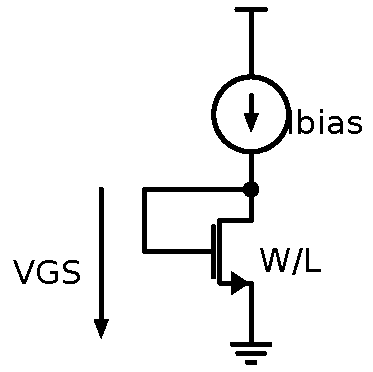
\includegraphics{index_files/mediabag/index_files/figure-pdf/fig-mosfet-diode-output-1.pdf}

}

\caption{\label{fig-mosfet-diode}A MOSFET connected as a diode.}

\end{figure}%

\textsubscript{Source:
\href{https://iic-jku.github.io/analog-circuit-design/index.qmd.html}{Article
Notebook}}

\subsection{Transistor Sizing Using gm/ID
Methodoloy}\label{transistor-sizing-using-gmid-methodoloy}

When designing circuits it is an important question how to select
various parameters of a MOSFET, like \(W\), \(L\), or the bias current
\(I_\mathrm{D}\). As a very practical approach we select the
\(g_\mathrm{m}/I_\mathrm{D}\) methodoloy introduced by P. Jespers and B.
Murmann in (Jespers and Murmann 2017). A brief introduction is available
\href{https://github.com/iic-jku/analog-circuit-design/blob/main/sizing/Ref_Murmann_gmID.pdf}{here}
as well.

\textsubscript{Source:
\href{https://iic-jku.github.io/analog-circuit-design/index.qmd.html}{Article
Notebook}}

\begin{figure}[H]

\centering{

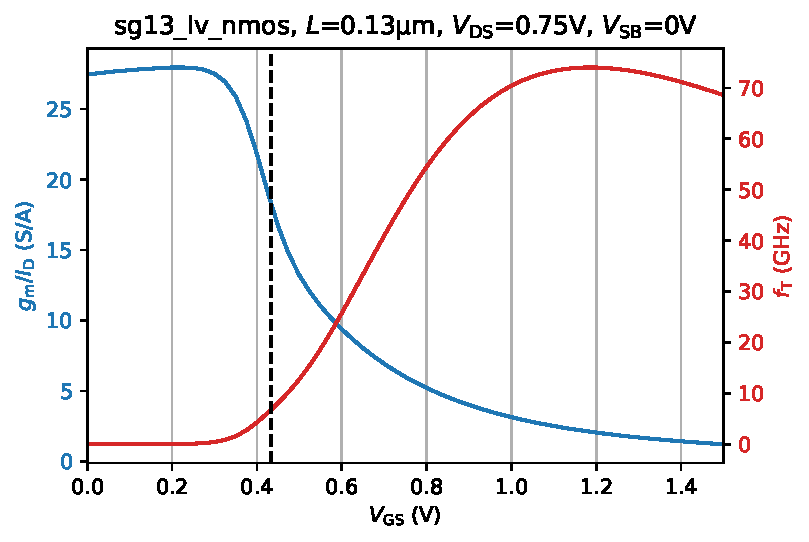
\includegraphics{index_files/figure-pdf/fig-nmos-gmid-vs-ft-output-1.pdf}

}

\caption{\label{fig-nmos-gmid-vs-ft}LV NMOS gm/ID vs.~transit
frequency.}

\end{figure}%

\textsubscript{Source:
\href{https://iic-jku.github.io/analog-circuit-design/index.qmd.html}{Article
Notebook}}

\begin{figure}[H]

\centering{

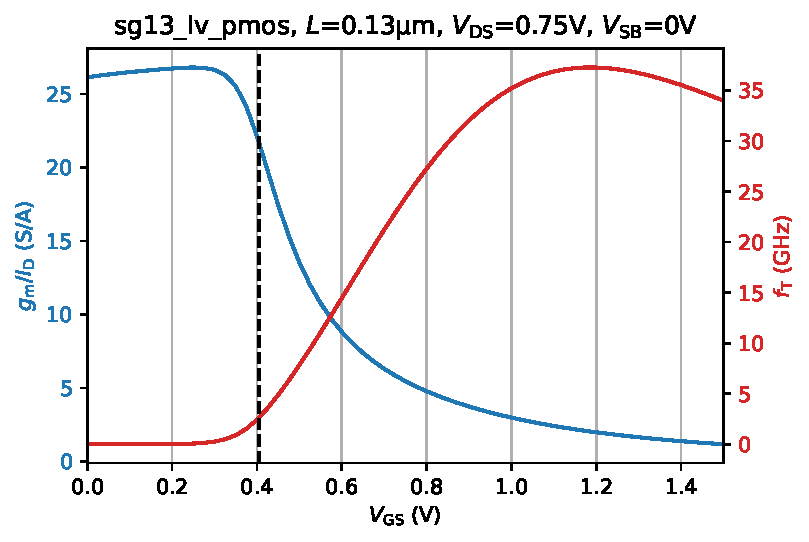
\includegraphics{index_files/figure-pdf/fig-pmos-gmid-vs-ft-output-1.pdf}

}

\caption{\label{fig-pmos-gmid-vs-ft}LV PMOS gm/ID vs.~transit
frequency.}

\end{figure}%

\textsubscript{Source:
\href{https://iic-jku.github.io/analog-circuit-design/index.qmd.html}{Article
Notebook}}

\subsection{Current Mirror}\label{current-mirror}

\subsection{Differential Pair}\label{differential-pair}

\subsection{Cascode Stage}\label{cascode-stage}

\subsection{A Basic 5-Transistor OTA}\label{a-basic-5-transistor-ota}

\subsection{A Fully-Differential OTA}\label{a-fully-differential-ota}

\subsection{Biasing the OTA}\label{biasing-the-ota}

\subsection{An RC-OPAMP Filter}\label{an-rc-opamp-filter}

\subsection{Summary \& Conclusion}\label{summary-conclusion}

\subsection{Appendix: ngspice Cheat
Sheet}\label{appendix-ngspice-cheat-sheet}

\subsection{Appendix: Xschem Cheat
Sheet}\label{appendix-xschem-cheat-sheet}

\textsubscript{Source:
\href{https://iic-jku.github.io/analog-circuit-design/index.qmd.html}{Article
Notebook}}

\phantomsection\label{refs}
\begin{CSLReferences}{1}{0}
\bibitem[\citeproctext]{ref-Jespers_Murmann_2017}
Jespers, Paul G. A., and Boris Murmann. 2017. \emph{Systematic Design of
Analog CMOS Circuits: Using Pre-Computed Lookup Tables}. Cambridge
University Press.

\end{CSLReferences}




\end{document}
